% !TeX encoding = UTF-8
%%%%%%%%%%%%%%%%%%%%%
%%%%% Anpassen! %%%%%
%%%%%%%%%%%%%%%%%%%%%
% Meta-Informationen 
\newcommand{\titel}{Community-basierte Wissensportale InDeKo.Navi Atlas}
\newcommand{\untertitel}{Installationsanleitung} 
\newcommand{\art}{Ausarbeitung}
\newcommand{\studiengang}{Wirtschaftsinformatik}
\newcommand{\autor}{Robin Helmedach, Konstantin Janzen, Friederike Lauterbach, Stephan Mende}
\newcommand{\email}{}
\newcommand{\matnr}{}
\newcommand{\institut}{Institut für Betriebswirtschaft und Wirtschaftsinformatik}
\newcommand{\arbeitsgruppe}{Arbeitsgruppe Informationssysteme und Unternehmensmodellierung}
\newcommand{\universitaet}{Universität Hildesheim \textbullet  Universitätsplatz 1 \textbullet  D-31134 Hildesheim}
\newcommand{\adresse}{\arbeitsgruppe  \textbullet  \institut \\ \universitaet}
\newcommand{\version}{Version 1.0}
\newcommand{\veranstaltung}{IT-Studienprojekt Master \\SoSe 2016 - WiSe 2016/2017}

%%%%%%%%%%%%%%%%%%%%%%%%%%%%%%%%%%%%%%%%%%%%%
%% Diese Datei muss nicht angepasst werden %%
%%%%%%%%%%%%%%%%%%%%%%%%%%%%%%%%%%%%%%%%%%%%%
% v1.3
%Schriftgröße, ein- oder zweiseitig, Papierformat, Dokumententyp
\documentclass[12pt,oneside,a4paper,bibliography=totoc,listof=totoc,
	ngerman,
	parskip=half, % Abstand zwischen Absätzen (halbe Zeile)
	headings=normal, % Größe der Überschriften verkleinern
	]{scrartcl}

%Seitenränder
\usepackage[left=2cm,right=2cm,top=2.5cm,bottom=2.5cm]{geometry}

%Neue Deutsche Rechtschreibung und Umlaute
\usepackage[T1]{fontenc}
\usepackage[utf8]{inputenc}
\usepackage[ngerman]{babel}
\usepackage[babel,german=quotes]{csquotes}
\usepackage{lmodern}
\usepackage[right]{eurosym}

\usepackage{caption}
\usepackage{subcaption}

%Kopf- und Fußzeile
\usepackage{fancyhdr}
\pagestyle{fancy} 
\fancyhf{}


\usepackage{lastpage}

\usepackage{tabularx}
\newcolumntype{L}[1]{>{\raggedright\arraybackslash}p{#1}} % linksbündig mit Breitenangabe
\newcolumntype{C}[1]{>{\centering\arraybackslash}p{#1}} % zentriert mit Breitenangabe
\newcolumntype{R}[1]{>{\raggedleft\arraybackslash}p{#1}} % rechtsbündig mit Breitenangabe

%Kopfzeile links bzw. innen
%\fancyhead[L]{\name}

%Kopfzeile mittig
%\fancyhead[R]{\thepage}

%Kopfzeile rechts bzw. außen
%\fancyhead[L]{\rightmark}

%Fußzeile
%\cfoot{\thepage}

% Kopfzeile und Fußzeile einstellen
%\textsc{\lhead{\name, \matrikel}
%\chead{\veranstaltung\ \ubungsnr}
%\rhead{\today}
\cfoot{\thepage\ / \pageref*{LastPage}}

%Linie oben / unten
\renewcommand{\headrulewidth}{0pt}
%\renewcommand{\footrulewidth}{0.5pt}



%Hübbsche Schriften im PDF-Viewer
\usepackage{ae}
\usepackage{times}


\usepackage{booktabs}

\makeatletter
\@ifpackageloaded{tex4ht}{%
      \usepackage[dvips]{graphicx}
      \usepackage[tex4ht]{hyperref}
    }{%

% Brauchbare PDF-Links und Angaben im PDF-Header
% Graphiken
\usepackage[pdftex]{graphicx}
\usepackage[hyphens]{url}
\PassOptionsToPackage{hyphens}{url}
\usepackage[ %pdftex,
	raiselinks=true,%
	bookmarks=true,%
	colorlinks=true,% Gibt man keine gedruckte Version ab, sondern das PDF, sollte man erwägen diesesn Wert auf "true" zu ändern
	linkcolor=black, % einfache interne Verknüpfungen
	anchorcolor=black, % Ankertext
	citecolor=black, % Verweise auf Literaturverzeichniseinträge im Text
	filecolor=black, % Verknüpfungen, die lokale Dateien öffnen
	menucolor=black, % Acrobat-Menüpunkte
	urlcolor=blue, 
	bookmarksopenlevel=1,%
	bookmarksopen=true,%
	bookmarksnumbered=true,%
	hyperindex=true,% 
	hypertexnames=false, % zur korrekten Erstellung der Bookmarks
	plainpages=false,% correct hyperlinks
	pdfpagelabels=true,% view TeX pagenumber in PDF reader
%%  pdfborder={0 0 0.5}
	pdfauthor={\autor},
	pdfsubject={\titel},
	pdfkeywords={},
	pdftitle={\titel},
	linktocpage = false, % Seitenzahlen anstatt Text im Inhaltsverzeichnis verlinken
	pdfstartview=FitH
]{hyperref}

}
\makeatother
%Thumbnails im PDF
%\usepackage{thumbpdf}
%hübschere Tabellenabstände
\usepackage{booktabs}

%diverser mathematischer Kram
\usepackage{amsmath}
\usepackage{amsthm}
\usepackage{amssymb}
\usepackage{multirow}

% Zitierstil
%\usepackage[round]{natbib}
%\usepackage[backend=biber, style=mla]{biblatex}
%\usepackage[backend=biber, style=apa]{biblatex}
%\usepackage[style=authoryear,natbib=true]{biblatex}
\usepackage[style=authoryear, maxnames=2, maxbibnames=99, backend=biber,firstinits=true, hyperref=true]{biblatex}
\DeclareNameAlias{sortname}{last-first}
%\DeclareLanguageMapping{ngerman}{ngerman-apa}



% Verhindern von "Schusterjungen" und "Hurenkindern"
\clubpenalty = 10000
\widowpenalty = 10000
\displaywidowpenalty = 10000
\tolerance=500 %Zeilenumbruch

% Abkürzungsverzeichnis
\usepackage[dua]{acronym}

%  Paket um ToDos einzufügen
\usepackage{todonotes}

%Für farbige Links
\usepackage{color, colortbl}
\definecolor{javared}{rgb}{0.6,0,0} % for strings
\definecolor{javagreen}{rgb}{0.25,0.5,0.35} % comments
\definecolor{javapurple}{rgb}{0.5,0,0.35} % keywords
\definecolor{javadocblue}{rgb}{0.25,0.35,0.75} % javadoc


\usepackage{listings}
\lstset{% general command to set parameter(s) 
frame=top,frame=bottom,
breaklines=true,
%basicstyle=\sffamily\footnotesize, % print whole listing small 
basicstyle=\verbatim@font\footnotesize,
keywordstyle=\color{javapurple}\bfseries, % ubold black keywords 
identifierstyle=, % nothing happens 
commentstyle=\color{javagreen}, % green comments 
stringstyle=\color{javared}, % typewriter type for strings 
morecomment=[s][\color{javadocblue}]{/**}{*/},
showstringspaces=false, % no special string spaces 
numbers=none, 
numberstyle=\sffamily\footnotesize, 
stepnumber=1, 
numbersep=10pt, 
showspaces=false, 
showtabs=false,
float=htbp, 
numberbychapter=true,
morekeywords={}
%columns=fullflexible, % can copy&paste listings
%language=R
} 
\renewcommand\lstlistingname{Code}

\usepackage{makeidx}
%\usepackage{url}
\usepackage{setspace}
\setlength{\parindent}{0pt} % Wie weit einrücken nach Absatz


%\usepackage{ulem}
\usepackage{enumerate}


\title{\titel}
\author{\autor}
\date{\today}

%\renewcommand{\topfraction}{0.85}
%\renewcommand{\textfraction}{0.1}

% Abstand Bild-Bildunterschrift
\setlength{\abovecaptionskip}{5pt plus 0pt minus 2pt} % Chosen fairly arbitrarily
\setlength{\belowcaptionskip}{5pt plus 0pt minus 2pt} % Chosen fairly arbitrarily

\usepackage{watermark}
%\renewcommand\arraystretch{1.3}% More space between table rows (MyValue=1.0 is for standard spacing)
\usepackage{array}
\newcolumntype{C}[1]{>{\centering\arraybackslash}m{#1}}

% Subliminal refinements towards typographical perfection
\usepackage{microtype}

% Intelligent cross-referencing
\usepackage[ngerman,nameinlink]{cleveref}

% Grafiken \ Plots
\usepackage{pgfplots,pgfplotstable}
\pgfplotsset{compat=1.11}
%\usepackage{tikz}
\usetikzlibrary{patterns}
\usetikzlibrary{intersections}
\usetikzlibrary{spy}
\usepgfplotslibrary{fillbetween}

% Pseudocode
\usepackage{algorithm}
\usepackage{algorithmicx}
\usepackage{algpseudocode}
%\usepackage{algorithm2e}

\usepackage{watermark}

\usepackage[clearempty]{titlesec}
% Einstellen der Schriftgrößen der Überschriften
\titleformat{\chapter}[hang]{\LARGE\bfseries}{\thechapter\quad}{0pt}{}
\titleformat{\section}[hang]{\Large\bfseries}{\thesection\quad}{0pt}{}
\titleformat{\subsection}[hang]{\large\bfseries}{\thesubsection\quad}{0pt}{}
\titleformat{\subsubsection}[hang]{\normalsize}{\thesubsubsection\quad}{0pt}{}

% Einstellen der Abstände vor und nach den Überschriften
\titlespacing{\subsubsection}{0pt}{0pt}{-5pt}

\usepackage{float}
\usepackage{enumitem}
%\usepackage[toc]{glossaries}
\selectlanguage{ngerman}

\newcommand*{\quelle}[1]{\par\raggedleft\scriptsize Quelle:~#1}
\DefineBibliographyStrings{german}{%
  andothers = {et al.},
}
%\addbibresource{atlas.bib}
\setlength\bibitemsep{5pt}  % Abstand zwischen 2 Einträgen im Verzeichnis

% Zeilenabstand: 1.5
\onehalfspacing

\renewcommand{\arraystretch}{1.2}
\urlstyle{same}

% hier wird ein neues Kommando definiert
\newcommand{\zB}{z.\,B. }
\newcommand{\noconfig}{Dieses Modul verfügt über kein Konfigurationsmenü oder veränderbare Einstellungen (deutsche Übersetzungen sowie das Übersetzungstemplate liegen bei).}
\newcommand{\standardinstall}{Dieses Modul lässt sich wie jedes andere Drupal Modul installieren.
	\begin{enumerate}
		\item Modul in das Custom-Module-Verzeichnis der Drupal-Installation kopieren  (\zB \lstinline|sites/all/modules/custom|, vgl. \cref{fig:structureproject})
		\item Modul auf der Seite \lstinline|admin/modules| aktivieren.
	\end{enumerate}}


%%%%% Einträge Glossar %%%%%
\newglossaryentry{imagemap}
{
	name=image map,
	plural=image maps,
	description={siehe \gls{verweissensitivegrafik}}
}
\newglossaryentry{verweissensitivegrafik}
{
	name=Verweissensitive Grafik,
	plural=Verweissensitive Grafiken,
	description={Verweis-sensitive Grafiken (englisch \textit{\glspl{imagemap}}) sind Grafiken, in denen der Anwender mit der Maus auf ein Detail klicken kann. Daraufhin wird ein Verweis ausgeführt. Auf diese Weise kann der Anwender in einigen Fällen wesentlich intuitiver und schneller zu Information gelangen als durch lange verbale Verweislisten.}
}
\newglossaryentry{wissenskarte}
{
	name=Wissenskarte,
	plural=Wissenskarten,
	description={(englisch \textit{knowledge map}) Visualisierung von Wissen}
}



%%%%%% Einträge Abkürzungsverzeichnis  %%%%%
\newacronym{indeko}{InDeKo}{Integratives demografiesensibles Kompetenzmanagement}


%%%%%%%%%%%%%%%%%%%%%%%%%%%%%%%%%%%
%%%%% Hier geht der Text los! %%%%%
%%%%%%%%%%%%%%%%%%%%%%%%%%%%%%%%%%%
\begin{document}


%\bibliographystyle{plainnat}
%\bibliographystyle{alpha}
\pagenumbering{roman}

% Erzeugt das Deckblatt
%   Bei zu langem Arbeitstitel müssen die vertikalen Abstände (\vspace)
%   angepasst werden, damit das Deckblatt weiterhin auf eine Seite passt.
\begin{titlepage}
\newgeometry{top=2cm,bottom=2cm,left=2cm,right=2cm}
\begin{figure}
	\centering
    \begin{minipage}{0.28\textwidth}
        \begin{flushleft}
            
\includegraphics[scale=0.23]{csm_ISUM_Logo_Final_107dd2fa79.jpg}
        \end{flushleft}
    \end{minipage}
    \begin{minipage}{0.35\textwidth}
        \centering
        \hspace{0.25cm}
    \end{minipage}
    \begin{minipage}{0.25\textwidth}
        \begin{flushright}
            
\includegraphics[scale=0.25]{St_Uni-Logo-9-2003-eps-converted-to.pdf}
        \end{flushright}
    \end{minipage}
    \vspace{4cm}
\end{figure}
\begin{center}

    \Huge{\textbf{\titel}}

    \Huge{\textbf{\untertitel}}
    \vspace{2cm}
\end{center}
\begin{center}
    \vspace*{0cm}
    \textbf{Ausarbeitung im Rahmen der Veranstaltung \veranstaltung}
    \vspace{1cm}
\end{center}
\begin{center}
    Institut für Betriebswirtschaft und Wirtschaftsinformatik,

    \arbeitsgruppe
\end{center}
\begin{center}
    \vspace{5cm}
    \autor\\


    \today
\end{center}
\end{titlepage}
\newpage


% Erzeugt das Inhaltsverzeichnis
\tableofcontents

% Erzeugt das Abbildungsverzeichnis
\newpage
\listoffigures
\thispagestyle{empty}


\newpage
\restoregeometry
\pagenumbering{arabic}




\section{Installation}
Dieses Kapitel beschreibt die Installation und Konfiguration des InDeKo.Navi Atlas Projekts.


\subsection{Installationsschritte}
\begin{enumerate}
	\item Vorausgesetzt werden mindestens ein Webserver der PHP unterstützt, PHP 5.2.5 sowie MySQL 5.0.15. Als Komplettpaket lässt sich \zB \href{https://www.apachefriends.org/de/download.html}{XAMPP} installieren (v5.6.12 empfohlen. In nachfolgenden Versionen wurde MySQL durch MariaDB ersetzt. Test der Installation verlief auch mit XAMPP 5.6.30 erfolgreich, aber entwickelt und getestet wurde ausschließlich mit MySQL).

	\item GitHub-Projekt herunterladen (Branch KnowledgeMap) \url{https://github.com/KonstantinJanzen/Atlas/tree/KnowledgeMap/}.
	Das Projekt enthält eine komplett konfigurierte Drupal 7.53 Installation.

	\item Inhalte des Atlas-Projekts in den Document Root (bzw. ein Unterverzeichnis, je nach gewünschter Konfiguration) des Webservers entpacken (\zB \textit{htdocs}, \textit{www})

	\item Drupal 7 Datenbank-Dump \textit{db\_wissenskarte.sql} aus dem Projekt-Unterordner \textit{sql\_dumps} importieren (hier beispielhaft für Datenbank Administrator \enquote{root} ohne Passwort):
	\begin{enumerate}
		\item \lstinline|mysqladmin -u root CREATE indeko|

		\item \lstinline|mysql -u root indeko < sql_dumps\db_wissenskarte.sql|
	\end{enumerate}

	\item Apache Solr Server installieren:
	\begin{enumerate}
		\item Apache Solr Version 5.5.2 herunterladen und entpacken \url{http://archive.apache.org/dist/lucene/solr/5.5.2/}.

		\item Aus dem Projekt-Unterordner \textit{solr\_config} den Ordner \textit{drupal} nach \lstinline|solr-5.5.2\server\solr\| kopieren.

		\item Solr Server starten (\zB \lstinline|solr-5.5.2\bin\solr start|).
		\item Der Apache Solr Server is lokal unter \url{http://localhost:8983/solr} zu erreichen.
	\end{enumerate}

	\item Apache Solr Suchindex in Drupal aktualisieren (\lstinline|admin/config/search/apachesolr|):
	\begin{enumerate}
		\item \enquote{Delete the Search \& Solr Index} $\rightarrow$ \enquote{Delete index}

		\item \enquote{Index all queued content}  $\rightarrow$ \enquote{Index all remaining}
	\end{enumerate}

	\item Das Portal kann nun genutzt werden.
	\begin{itemize}
		\item Administrator-Account \enquote{admin} mit Passwort \enquote{pw}
		\item Benutzer-Accounts \enquote{ruser}, \enquote{ruser2}, \enquote{ruser3}, \enquote{ruser4}, \enquote{ruser5}  mit Passwort \enquote{pw}
	\end{itemize}
\end{enumerate}



\section{Projektstruktur}
Dieses Kapitel beschreibt die grundsätzliche Struktur des Atlas Projekts. Alle Änderungen im Vergleich zum InDeKo.Navi Ausgangsprojekt sind hervorgehoben und beschrieben. \cref{sub:strukture_project} beschreibt die Struktur des Drupal-Projekts und \cref{sub:strukture_module} geht auf die Struktur der entwickelten Custom Module ein.


\subsection{Grundsätzliche Drupal-Strukur}\label{sub:strukture_project}
\begin{figure}[!h]
	\centering
	\begin{subfigure}[a]{0.4\textwidth}
		\centering
		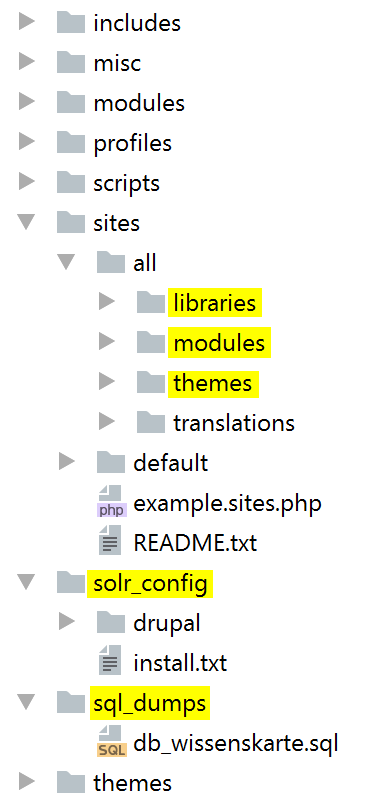
\includegraphics[height=0.25\textheight]{images/structure_project}
		\caption[]{Drupal-Projekt}
		\label{fig:structureproject}
	\end{subfigure}
	%
	\begin{subfigure}[A]{0.4\textwidth}
		\centering
		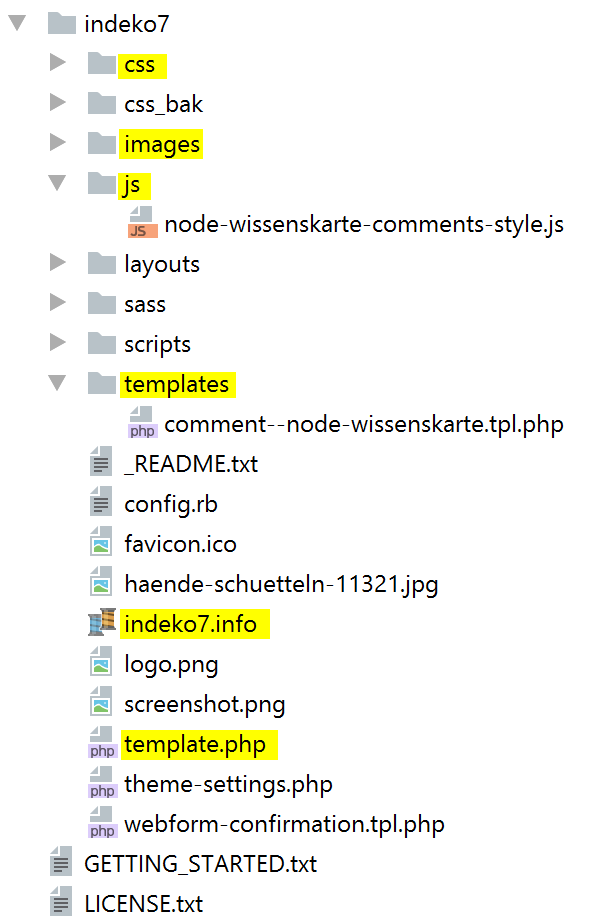
\includegraphics[height=0.25\textheight]{images/structure_theme}
		\caption[]{indeko7 Theme}
		\label{fig:structuretheme}
	\end{subfigure}
	\caption{Grundstruktur des Drupal-Projekts}
	\label{fig:structure}
\end{figure}


\cref{fig:structureproject} stellt die grundsätzliche Struktur des Drupal-Projekts dar:
\begin{itemize}
	\item \textit{libraries}: Enthält zusätzlich installierte externe Javascript Bibliotheken (\zB\ Chosen, qTip2).

	\item \textit{modules}: Der Unterordner \textit{custom} enthält alle entwickelten Module.

	\item \textit{themes}: Enthält alle installierten Drupal-Themes. Für das Projekt relevant ist das adaptivetheme indeko7 (siehe \cref{fig:structuretheme}).

	\item \textit{solr\_config}: Enthält Konfigurationsdateien für den Apache Solr Server. \textit{install.txt} beschreibt die Installation im Detail.

	\item \textit{sql\_dumps}: Enthält den Datanbank-Dump des InDeKo.Navi Atlas-Projekts  (\textit{db\_wissenskarte.sql}).
\end{itemize}



\cref{fig:structuretheme} stellt die Hauptstruktur des indeko7 Themes dar (\lstinline|\sites\all\themes\adaptivetheme\indeko7|):
\begin{itemize}
	\item \textit{css}: Enthält .css Dateien, die das grundlegende Design betreffen. Alle das Portal betreffenden Änderungen sind in der Datei \textit{global.atlas.css} zusammengefasst.

	\item \textit{images}: Der Unterordner \textit{atlas} enthält Bilddateien, die speziell für das Atlas-Projekt entworfen wurden und in den .css Dateien verwendet werden (\zB spezifische Icons für Inhaltstypen oder Aktionen).

	\item \textit{js}: Enthält .js Dateien, die ausschließlich das Design betreffen.

	\item \textit{templates}: Enthält Template-Dateien (.tpl.php), die gezielt die Darstellung der Inhalte des Portals steuern.

	\item \textit{indeko7.info}: Enthält einen zusätzlichen Eintrag, um \textit{global.atlas.css} einzubinden

	(\lstinline|stylesheets[screen][] = css/global.atlas.css|).

	\item \textit{template.php}: Enthält Logik, die die von Drupal bereitgestellten Informationen zur Darstellung der Inhalte anpasst.

\end{itemize}



\subsection{Grundsätzliche Modulstruktur}\label{sub:strukture_module}
\begin{figure}
	\centering
	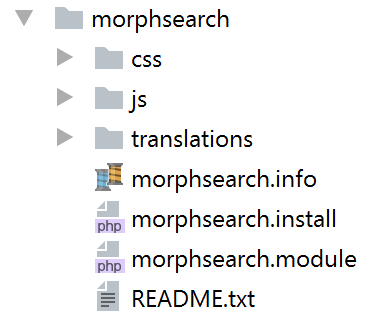
\includegraphics[height=0.2\textheight]{images/structure_module}
	\caption{Grundstruktur Custom Modul}
	\label{fig:structuremodule}
\end{figure}

Dieser Abschnitt beschreibt die grundsätzliche Struktur der entwickelten Custom Module (\lstinline|\sites\all\modules\custom|):

\begin{itemize}
	\item \textit{css}: Enthält CSS Dateien, die speziell das Modul betreffen.

	\item \textit{js}: Enthält JavaScript Dateien, die speziell das Modul betreffen.

	\item \textit{translations}: Enthält eine Übersetzungs-Vorlage (.pot), die alle übersetzbaren Texte des Moduls enthält und eine deutsche Übersetzungsdatei (.de.po). Die Übersetzungen werden während der Installation des Moduls importiert oder können jederzeit manuell in Drupal importiert werden (\lstinline|admin/config/regional/translate/import|). Templates erstellt mit dem Translation template extractor Modul (\url{https://www.drupal.org/project/potx})

	\item \textit{.info}: Enthält Informationen über das Modul, die von Drupal benötigt werden (Abhängigkeiten, Menüs, \dots).

	\item \textit{.install}: Enthält Installations- und Deinstallationsroutinen (Variablen, Datenbank-Tabellen und Einträge).

	\item \textit{.module}: Enthält den PHP Quellcode des Moduls.

	\item \textit{README.txt}: Enthält die Beschreibung des Moduls, die Installationsanleitung inklusive Pflicht- und optionaler Module, sowie eine Beschreibung der Konfiguration (in Anlehnung an das Drupal README Template \url{https://www.drupal.org/node/2181737}).
\end{itemize}




\section{Anmerkungen zum Produktivbetrieb}\label{sec:live}
Dieser Abschnitt enthält Punkte, die bei der Überführung des InDeKo.Navi-Portals aus der Test-Umgebung in eine Live-Umgebung beachtet werden sollten.

\begin{itemize}
	\item In der Entwicklung genutzte Benutzeraccounts deaktivieren, da die Passwörter unsicher sind (\lstinline|admin/people|): \enquote{admin}, \enquote{ruser}, \enquote{ruser2}, \enquote{ruser3}, \enquote{ruser4}, \enquote{ruser5}.

	\item Beispiel-Wissenskarten löschen, da nicht geprüft wurde, ob die verwendeten Bilder lizenzfrei sind (\lstinline|admin/content|, siehe \cref*{sub:license} \cref{sub:license_images}).

	\item Für den CSV-Export der Suchergebnisse, die aus dem Internet erreichbare URL des Apache Solr Servers eintragen (\lstinline|admin/config/morphsearch_csv_export|).

	\item Anzuzeigende Fehlermeldungen deaktivieren (\lstinline|admin/config/development/logging|).

	\item \dots \todo{was noch?
    - Projekte, Publikationen, FEs, die als Test angelegt wurden noch löschen
    - Benutzer wie "Dagobert Duck", "Miss Piggy" etc. löschen}
    huhu
\end{itemize}



\newpage
\section{Funktionalität}\label{sec:function}
Dieses Kapitel beschreibt die im Laufe des Projekts entwickelten Funktionalitäten. \cref{sub:custom_modules} beschäftigt sich mit den entstandenen Custom Modulen. \cref{sub:drupal_customizing} beschreibt Funktionalitäten, die ausschließlich durch den Einsatz von Contributed oder Drupal-Core Modulen und Customizing in Drupal umgesetzt wurden.


\subsection{Entwickelte Custom Module}\label{sub:custom_modules}


\begin{figure}[H]
	\centering
	\begin{subfigure}{0.45\textwidth}
		\centering
		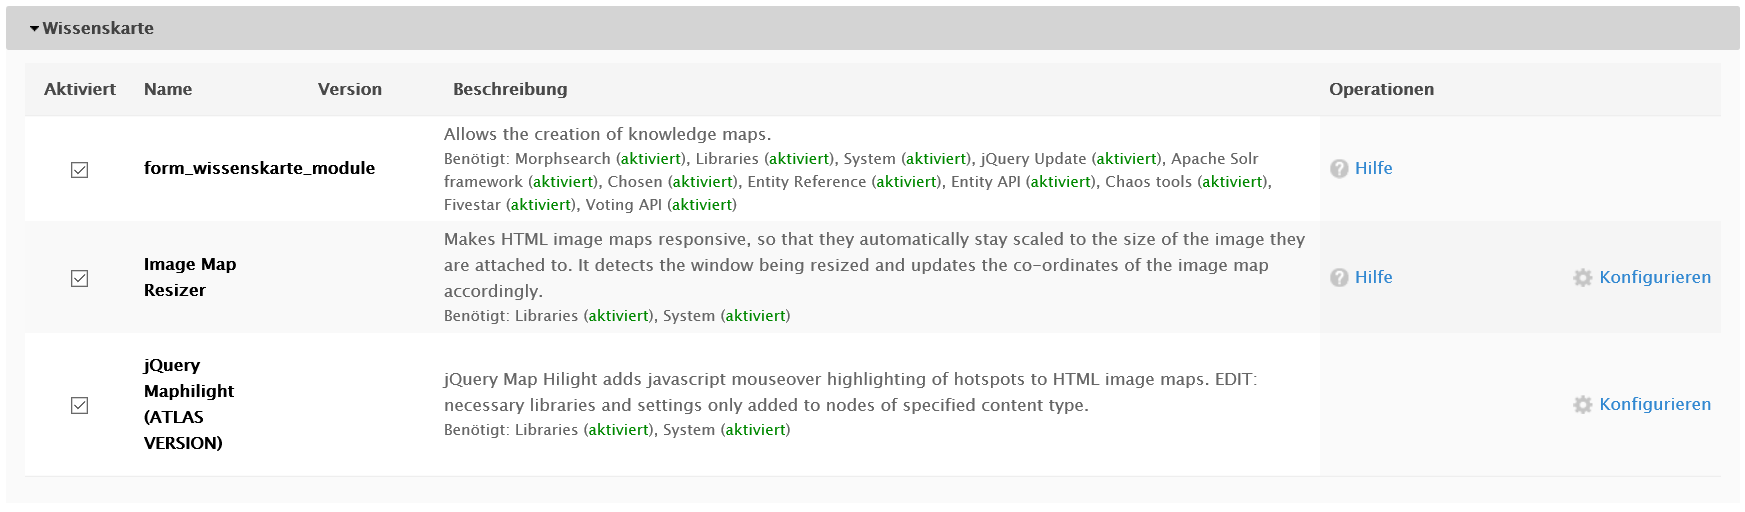
\includegraphics[width=0.95\linewidth]{images/modules_knowledgemap}
		\caption{Module Wissenskarte}
		\label{fig:modules_knowledgemap}
	\end{subfigure}
	%
	\begin{subfigure}{0.45\textwidth}
		\centering
		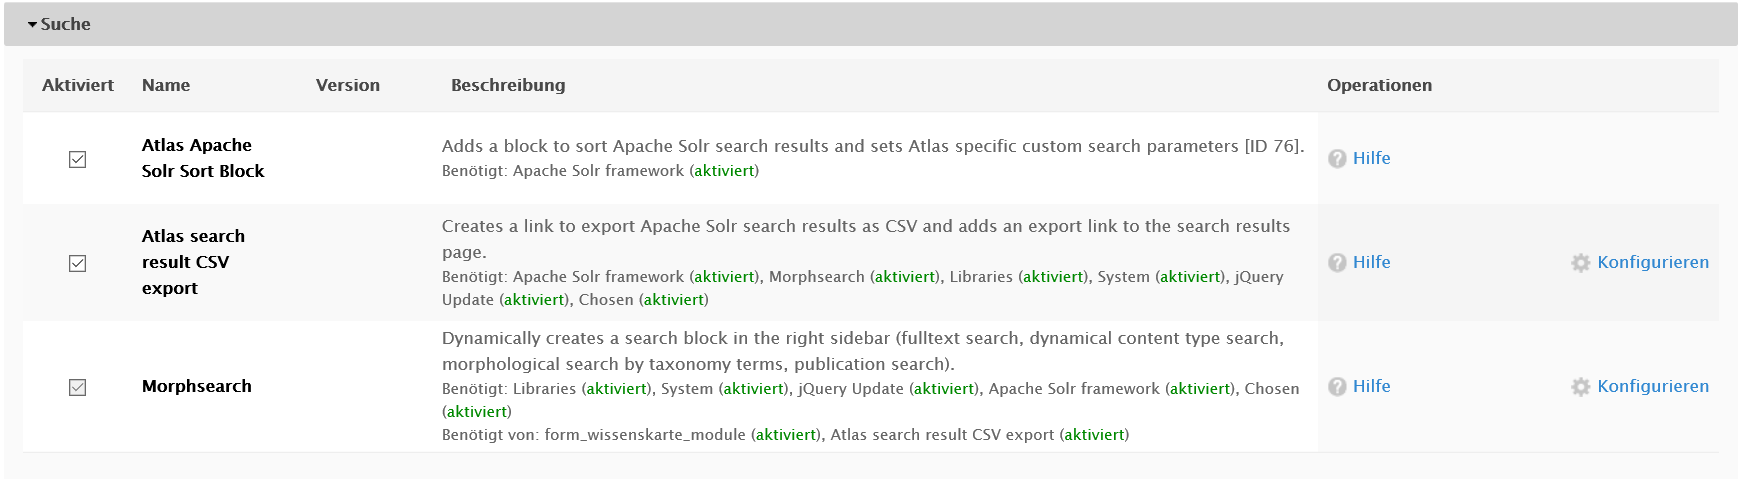
\includegraphics[width=0.95\linewidth]{images/modules_search}
		\caption{Module Suche}
		\label{fig:modules_search}
	\end{subfigure}
	\begin{subfigure}{0.45\textwidth}
		\centering
		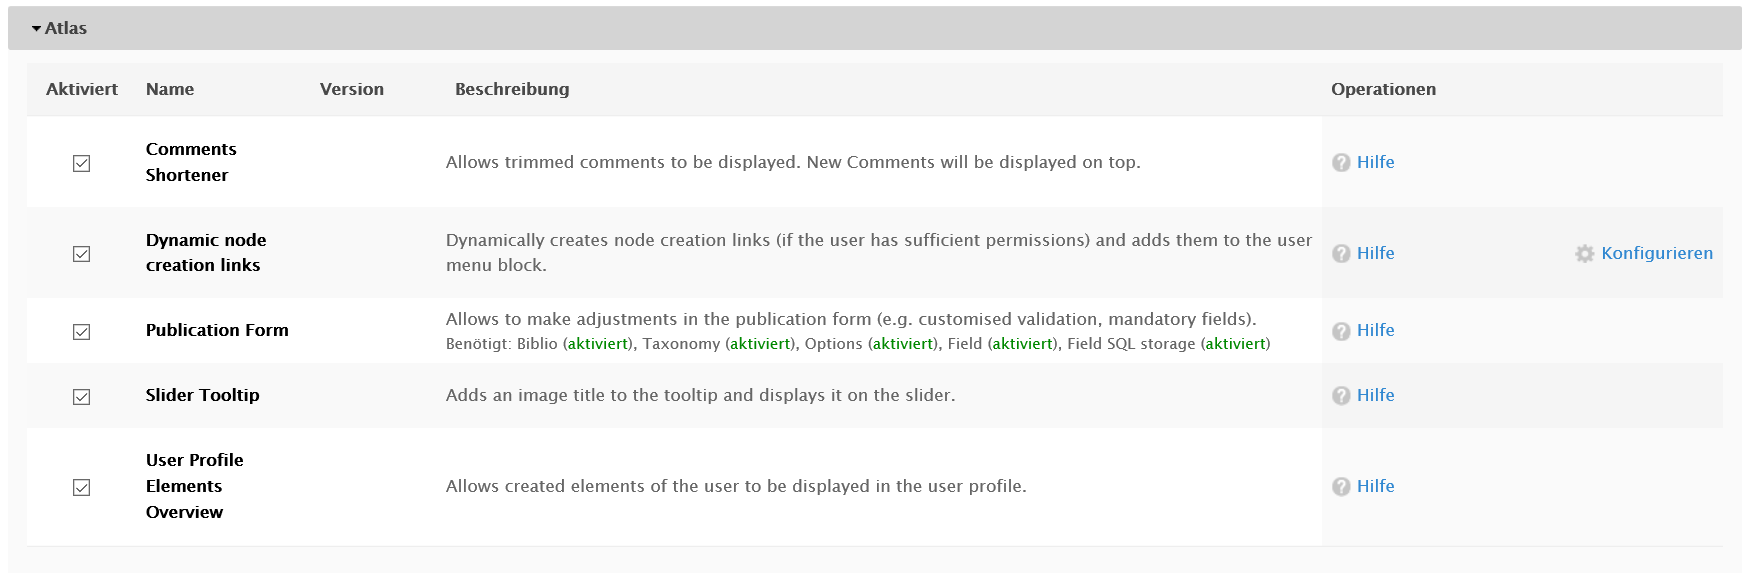
\includegraphics[width=0.95\linewidth]{images/modules_atlas}
		\caption{Module Atlas}
		\label{fig:modules_atlas}
	\end{subfigure}
	\caption{Entwickelte Custom Module}
	\label{fig:modules_all}
\end{figure}

Dieser Abschnitt beschreibt die im Laufe des Projekts entwickelten Drupal Custom Module. Diese Module wurden in die Bereiche Wissenskarte (siehe \cref{fig:modules_knowledgemap}), Suche (siehe \cref{fig:modules_search}), sowie Atlas für allgemeine Module (siehe \cref{fig:modules_atlas}) unterteilt.
Für jedes Modul wird der Funktionsumfang kurz beschrieben sowie auf die Punkte \enquote{Vorausgesetzte Module}, \enquote{Empfohlene Module}, \enquote{Installation} und \enquote{Konfiguration} eingegangen. \enquote{Vorausgesetzte Module} listet alle Module, die zusätzlich zum entwickelten Modul installiert sein müssen, auf. Diese Informationen sind auch in den README.txt und den [Modul].info Dateien hinterlegt (somit wird man bei der Installation auch von Drupal auf fehlende vorausgesetzte Module hingewiesen). Der Punkt \enquote{Empfohlene Module} listet Module auf, die nicht zwingend benötigt werden, aber zum Nutzen des entwickelten Moduls beitragen. Unter \enquote{Installation} werden alle nötigen Installationsschritte aufgeführt und \enquote{Konfiguration} erläutert mögliche Einstellungen am Modul bzw. das Konfigurationsmenü. Alle Texte der Module sind englisch. Jedem Modul liegen im Unterordner \enquote{translations} jeweils ein Übersetzungstemplate (mit allen übersetzbaren Textstellen) sowie eine deutsche Übersetzung bei. Diese ermöglichen bei aktiviertem Drupal-Core Modul \enquote{locale} die Konfiguration der Sprache (\lstinline|admin/config/regional/translate|, importieren oder Textstellen manuell übersetzen).






\newpage
\subsubsection{form\_wissenskarte\_module}\label{subsub:form_wissenskarte_module}
Dieses Modul ermöglicht es Benutzern \glspl{verweissensitivegrafik} (engl. \glspl{imagemap}) aus Bilddateien (.jpg, .png) zu erstellen. Hierzu wird bei der Installation ein neuer Inhaltstyp \enquote{Wissenskarte} erstellt. Dies ermöglicht es Bilder auf das Drupal-Portal zu übertragen und auf diesen geometrische Bereiche einzuzeichnen. Diese Bereiche können mit Informationen aus dem Drupal-Portal angereichert und anderen Benutzern zugänglich gemacht werden.

\begin{figure}[H]
	\centering
	\begin{subfigure}{0.45\textwidth}
		\centering
		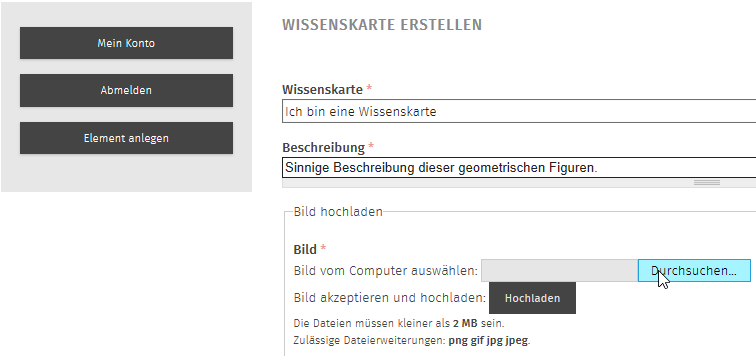
\includegraphics[width=0.95\linewidth]{images/example_knowledgemap_upload}
		\caption[]{Beispiel Wissenskarte hochladen}
		\label{fig:example_wissenskarte_upload}
	\end{subfigure}
	%
	\begin{subfigure}{0.45\textwidth}
		\centering
		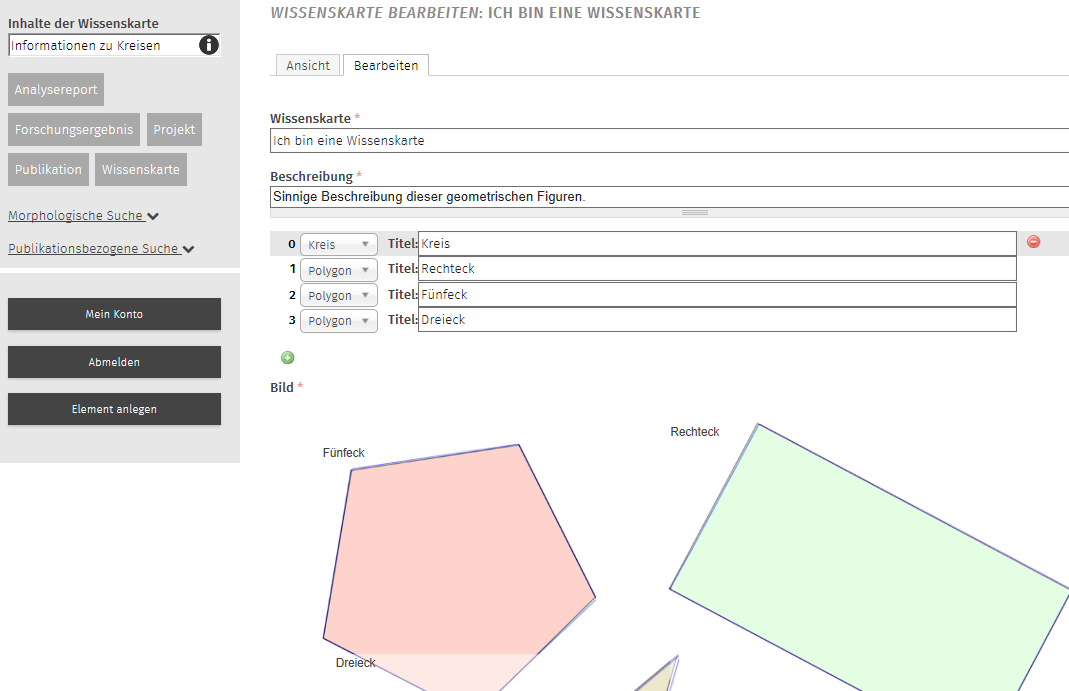
\includegraphics[width=0.95\linewidth]{images/example_knowledgemap_edit}
		\caption[]{Beispiel Wissenskarte bearbeiten}
		\label{fig:example_wissenskarte_edit}
	\end{subfigure}
	\caption{Custom Modul form\_wissenskarte\_module}
	\label{fig:example_form_wissenskarte_module}
\end{figure}

\begin{itemize}[parsep=0pt, itemsep=5.0pt plus 2.0pt minus 1.0pt, leftmargin=*]
	\item Vorausgesetzte Module:

	morphsearch (siehe \cref{subsub:morphsearch}): Wird genutzt, um die Inhalte der gezeichneten Bereiche auszuwählen.


	\item Empfohlene Module:

	Entityreference (\url{https://www.drupal.org/project/entityreference}): Ist dieses Modul installiert, werden alle Informationen, die den einzelnen Bereichen der Wissenskarte zugeordnet sind, auch mit der gesamten Wissenskarte verknüpft. Ansonsten lassen sich Wissenskarten nur über Titel und Beschreibung per Suche finden.

	Fivestar (\url{https://www.drupal.org/project/fivestar}): Ermöglicht es Benutzern Wissenskarten zu bewerten.


	\item Installation: \standardinstall


	\item Konfiguration:

	\noconfig

	Alle nötigen Einstellungen werden automatisch bei der Installation durchgeführt (.install Datei).

	Dieses Modul identifiziert Wissenskarten durch, der Bilddatei zugeordnete, Bildstile (\zB CSS-Klasse \enquote{image-style-wissenkarte}). Das verwendete Theme muss diese CSS-Klassen im HTML zur Verfügung stellen (beim Drupal 7 Standard Theme ist dies nicht der Fall).
\end{itemize}



\subsubsection{comments\_shortener}\label{subsub:commentsshortener}
Dieses Modul passt das Standard-Verhalten der Drupal Kommentarsektion an:

\begin{enumerate}
	\item Kommentare werden auf maximal 50 Zeichen gekürzt. Gekürzte Kommentare werden durch Auslassungspunkte am Ende kenntlich gemacht (siehe \cref{fig:example_commentshortener_short}). Ein Klick auf die Auslassungspunkte zeigt den vollständigen Kommentar an (siehe \cref{fig:example_commentshortener_full}).

	\item Neueste Kommentare werden zuerst angezeigt (dies ließ sich nicht über Drupal-Core Einstellungen konfigurieren).

	\item Nachdem ein Kommentar abgegeben wurde, wird der Benutzer auf die erste Kommentarseite zurückgeleitet (dies ließ sich nicht über Drupal-Core Einstellungen konfigurieren).
\end{enumerate}

\begin{figure}[H]
	\centering
	\begin{subfigure}{0.45\textwidth}
		\centering
		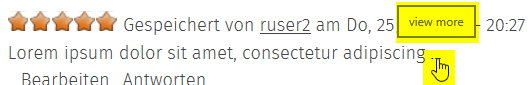
\includegraphics[width=0.95\linewidth]{images/example_commentsshortener}
		\caption[]{Beispiel gekürzte Darstellung}
		\label{fig:example_commentshortener_short}
	\end{subfigure}
	%
	\begin{subfigure}{0.45\textwidth}
		\centering
		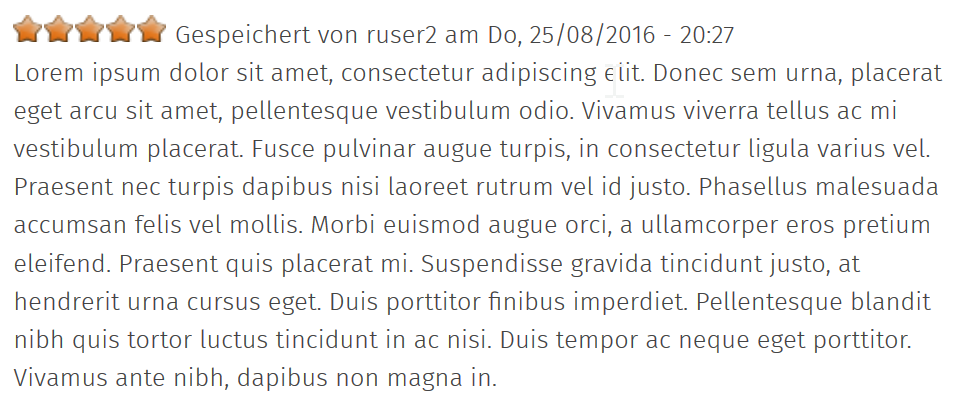
\includegraphics[width=0.95\linewidth]{images/example_commentsshortener_full}
		\caption[]{Beispiel Volldarstellung}
		\label{fig:example_commentshortener_full}
	\end{subfigure}
	\caption{Custom Modul comments\_shortener}
	\label{fig:example_commentsshortener}
\end{figure}

\begin{itemize}[parsep=0pt, itemsep=5.0pt plus 2.0pt minus 1.0pt, leftmargin=*]
	\item Vorausgesetzte Module:

	keine


	\item Empfohlene Module:

	form\_wissenskarte\_module (siehe \cref{subsub:form_wissenskarte_module}): Das comments\_shortener Modul ist auf die Anforderungen von Wissenskarten zugeschnitten, funktioniert aber auch ohne dieses Modul für jede Art von Kommentar.


	\item Installation: \standardinstall

	\item Konfiguration:

	\noconfig

\end{itemize}



\newpage
\subsubsection{imagemap\_resizer}\label{subsub:imagemapresizer}
Dieses Modul sorgt dafür, dass \textit{\glspl{imagemap}} \textit{responsive} werden. Die gezeichneten Konturen werden automatisch an die aktuelle Darstellungsgröße der \textit{\gls{imagemap}} angepasst (siehe \cref{fig:example_imagemapresizer}).

\begin{figure}[H]
	\centering
	\begin{subfigure}{0.45\textwidth}
		\centering
		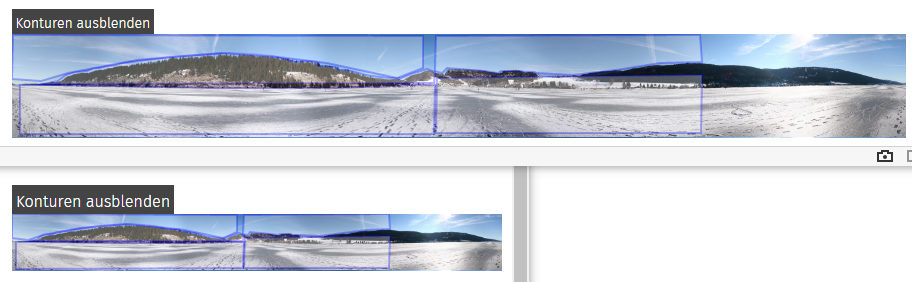
\includegraphics[width=0.95\linewidth]{images/example_imagemapresizer}
		\caption[]{Beispiel}
		\label{fig:example_imagemapresizer}
	\end{subfigure}
	%
	\begin{subfigure}{0.45\textwidth}
		\centering
		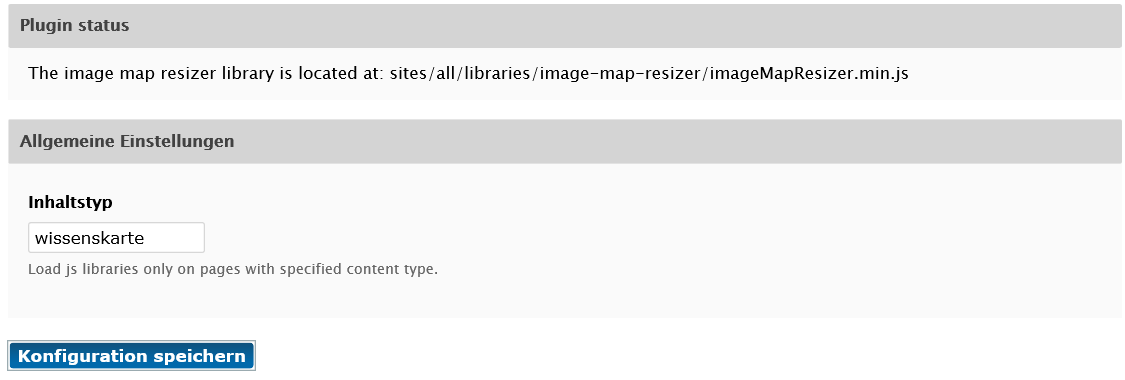
\includegraphics[width=0.95\linewidth]{images/config_imagemapresizer}
		\caption[]{Konfigurationsmenü}
		\label{fig:config_imagemapresizer}
	\end{subfigure}
	\caption{Custom Modul imagemap\_resizer}
	\label{fig:imagemap_resizer}
\end{figure}

\begin{itemize}[parsep=0pt, itemsep=5.0pt plus 2.0pt minus 1.0pt, leftmargin=*]
	\item Vorausgesetzte Module:

	Libraries (\url{https://www.drupal.org/project/libraries})


	\item Empfohlene Module:

	form\_wissenskarte\_module (siehe \cref{subsub:form_wissenskarte_module}): Legt den Inhaltstyp \textit{wissenskarte} an und ermöglicht es \textit{\glspl{imagemap}} selbst zu erzeugen.

	\item Installation:
	\begin{enumerate}
		\item Place it in the custom modules directory for your site (vgl. \cref{fig:structureproject}, e.g. \lstinline|sites/all/modules/custom|)
		\item Download the Image Map resize plugin from \url{https://github.com/davidjbradshaw/image-map-resizer}
		\item Extract the \textit{imageMapResizer.min.js} file into the \lstinline|sites/all/libraries/image-map-resizer| directory.
		\item Enable it on the \lstinline|admin/modules| page.
		\item Set the content type that contains \textit{\glspl{imagemap}} and should be resized on the configuration page \lstinline|admin/config/imagemap_resizer| (siehe \cref{fig:config_imagemapresizer}).
	\end{enumerate}


	\item Konfiguration:

	\cref{fig:config_imagemapresizer} stellt das Konfigurationsmenü dar. Im ersten Abschnitt lässt sich der Status der externen JavaScript Bibliothek ablesen. In dem darauffolgenden Textfeld wird der Maschinenname des Inhaltstyps angegeben, der Wissenskarten enthält. Die für die Skalierung von Wissenskarten benötigten JavaScript Dateien werden nur auf Seiten des angegebenen Inhaltstyps geladen. Als Standardwert ist der von dem Custom Modul form\_wissenskarte\_module (\cref{subsub:form_wissenskarte_module}) erstellte Inhaltstyp \textit{wissenskarte} definiert.

\end{itemize}



\newpage
\subsubsection{jq\_maphilight}\label{subsub:maphilight}
jq\_maphilight
\begin{figure}[H]
	\centering
	\begin{subfigure}[a]{0.4\textwidth}
		\centering
		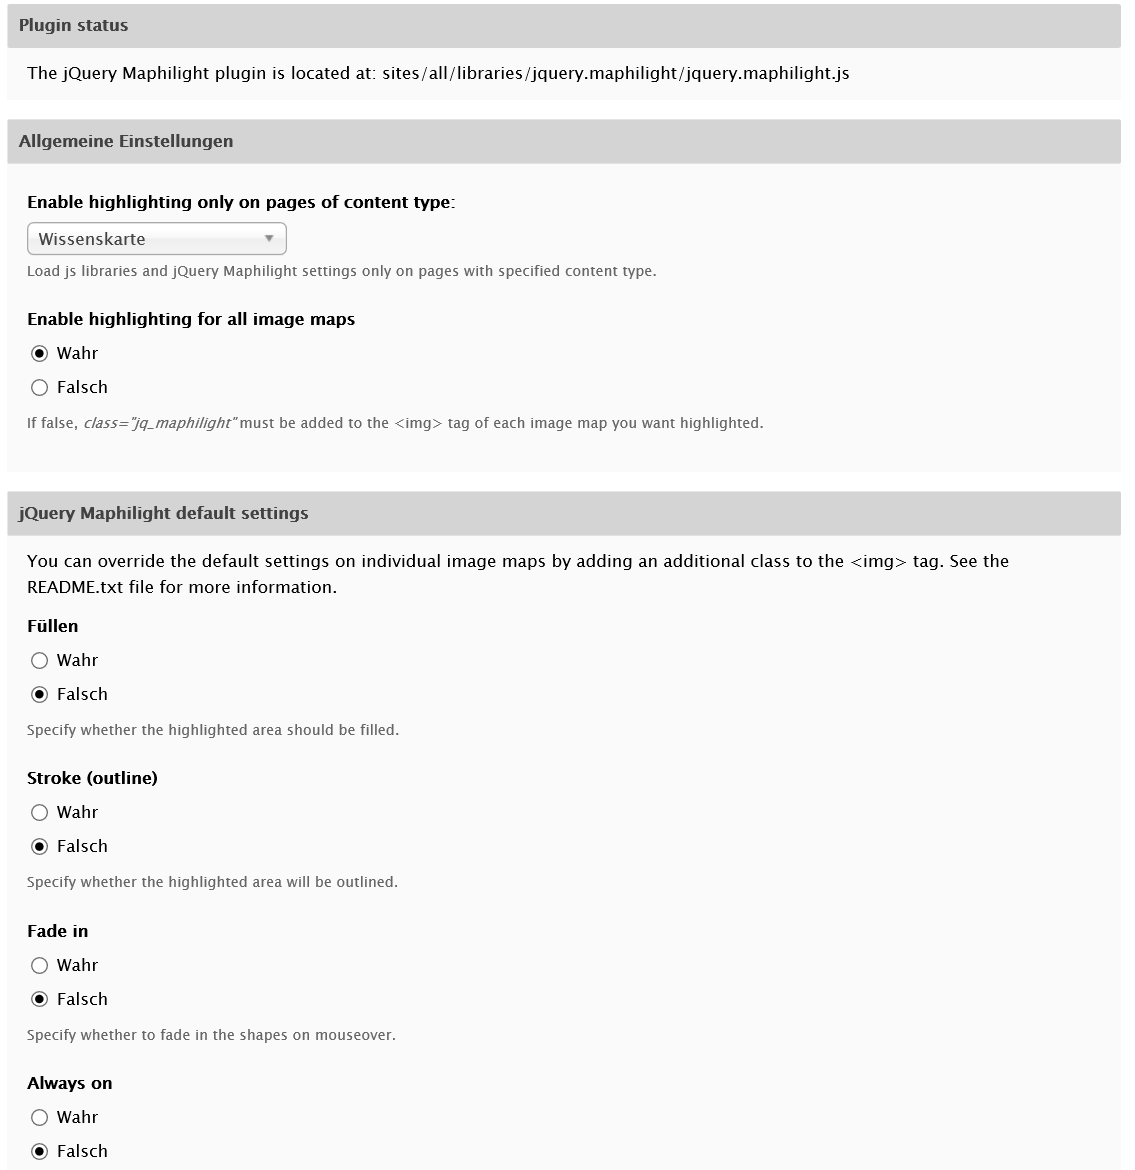
\includegraphics[height=0.20\textheight]{images/config_maphilight1}
		\caption[]{Allgemeine Einstellungen}
		\label{fig:config_maphilight1}
	\end{subfigure}
	%
	\begin{subfigure}[A]{0.4\textwidth}
		\centering
		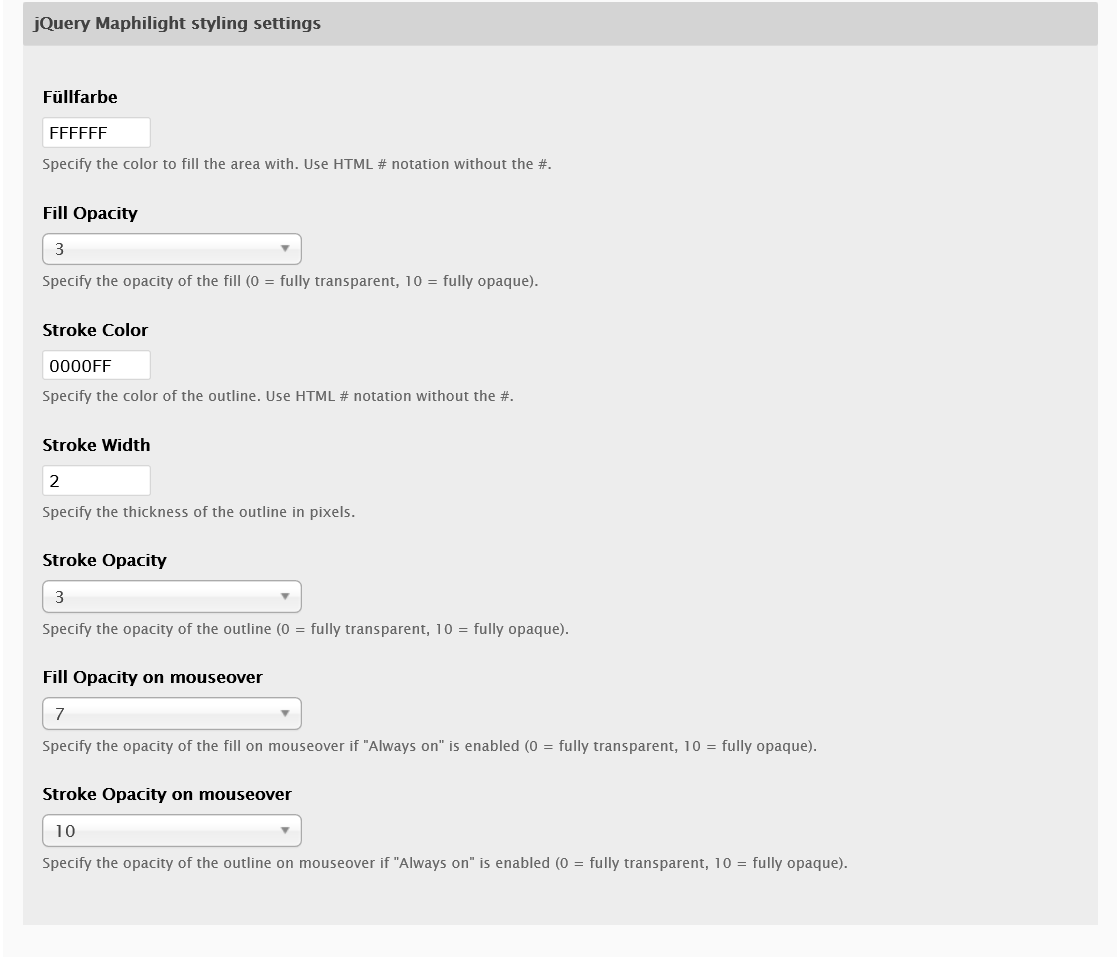
\includegraphics[height=0.20\textheight]{images/config_maphilight2}
		\caption[]{Styling Einstellungen}
		\label{fig:config_maphilight2}
	\end{subfigure}
	\caption{Konfigurationsmenü jq\_maphilight}
	\label{fig:config_maphilight}
\end{figure}

\begin{itemize}[parsep=0pt, itemsep=5.0pt plus 2.0pt minus 1.0pt, leftmargin=*]
	\item Vorausgesetzte Module:

	\item Empfohlene Module:

	\item Installation: \standardinstall

	\item Konfiguration:

\end{itemize}



\newpage
\subsubsection{morphsearch}\label{subsub:morphsearch}
morphsearch
\begin{figure}[H]
	\centering
	\begin{subfigure}[a]{0.45\textwidth}
		\centering
		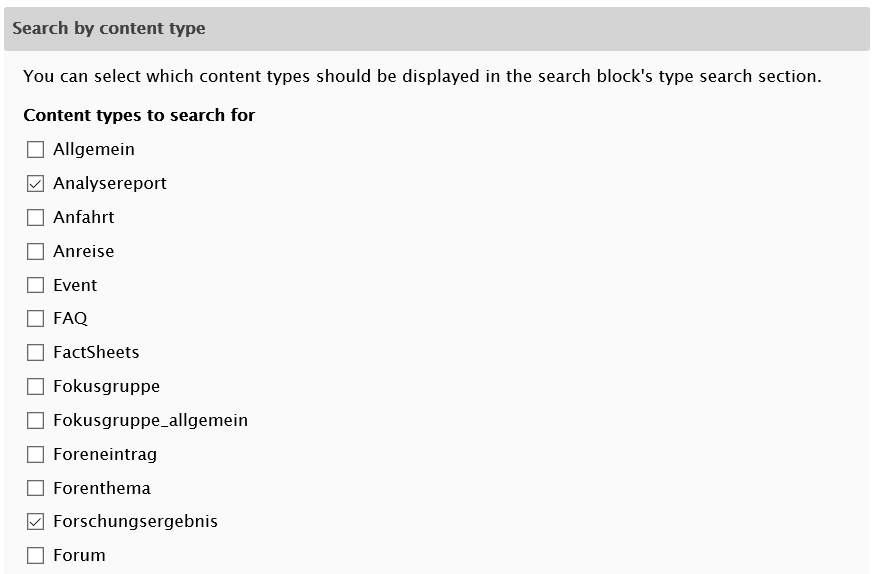
\includegraphics[height=0.20\textheight]{images/config_morphsearch}
		\caption[]{Konfigurationsmenü}
		\label{fig:config_morphsearch}
	\end{subfigure}
	%
	\begin{subfigure}[A]{0.25\textwidth}
		\centering
		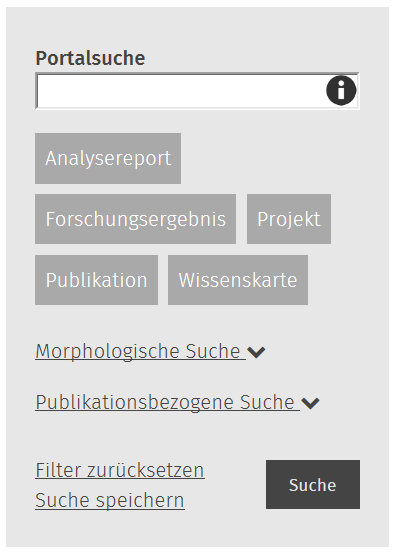
\includegraphics[height=0.20\textheight]{images/example_morphsearch}
		\caption[]{Beispiel}
		\label{fig:example_morphsearch}
	\end{subfigure}
	\caption{Custom Modul morphsearch}
	\label{fig:morphsearch}
\end{figure}



\subsubsection{morphsearch\_csv\_export}\label{subsub:morphsearchcsv}
morphsearch\_csv\_export
\begin{figure}[H]
	\centering
	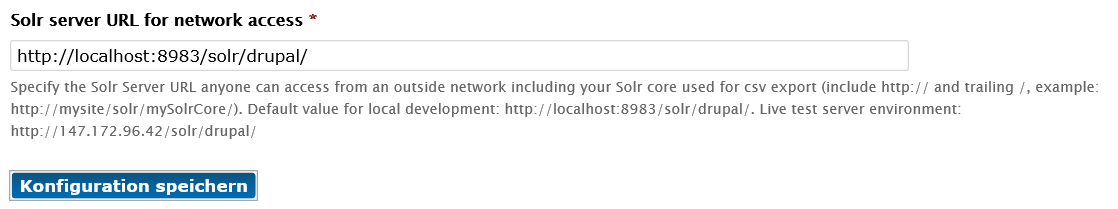
\includegraphics[width=0.70\linewidth]{images/config_searchcsv}
	\caption{Konfigurationsmenü morphsearch\_csv\_export}
	\label{fig:config_search}
\end{figure}



\newpage
\subsubsection{morphsearch\_sort}\label{subsub:morphsearchsort}
Dieses Modul fügt der Drupal-Installation einen Block hinzu, der es erlaubt Apache Solr Suchergebnisse zu sortieren. Es lässt sich nach Relevanz, sowie Datum und Titel (jeweils auf- und absteigend) sortieren (siehe \cref{fig:example_morphsearchsort}).


\begin{figure}[H]
	\centering
	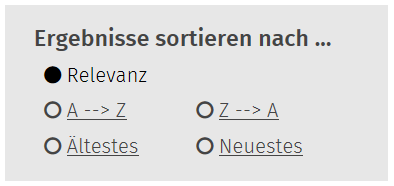
\includegraphics[height=0.10\textheight]{images/example_morphsearchsort}
	\caption{Custom Modul morphsearch\_sort Beispiel}
	\label{fig:example_morphsearchsort}
\end{figure}

\begin{itemize}[parsep=0pt, itemsep=5.0pt plus 2.0pt minus 1.0pt, leftmargin=*]
	\item Vorausgesetzte Module:

	Apache Solr Search (\url{https://www.drupal.org/project/apachesolr})


	\item Empfohlene Module:

	morphsearch (siehe \cref{subsub:morphsearch}): Ermöglicht es die zu sortierenden Suchergebnisse einzuschränken.


	\item Installation: \standardinstall

	\item Konfiguration:

	\noconfig

	Das Aussehen des Sortierblocks wird per CSS im Theme definiert (\zB \textit{drupal.atlas.css}, siehe \cref{sub:strukture_project}).

\end{itemize}


\newpage
\subsubsection{node\_creation\_links}\label{subsub:nodecreationlinks}
node\_creation\_links
\begin{figure}[H]
	\centering
	\begin{subfigure}[a]{0.4\textwidth}
		\centering
		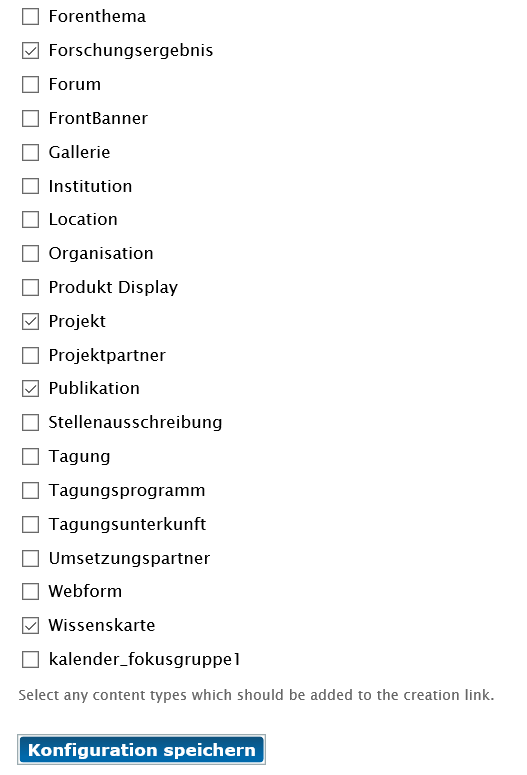
\includegraphics[height=0.20\textheight]{images/config_nodecreationlinks}
		\caption[]{Konfigurationsmenü}
		\label{fig:config_nodecreationlinks}
	\end{subfigure}
	%
	\begin{subfigure}[A]{0.4\textwidth}
		\centering
		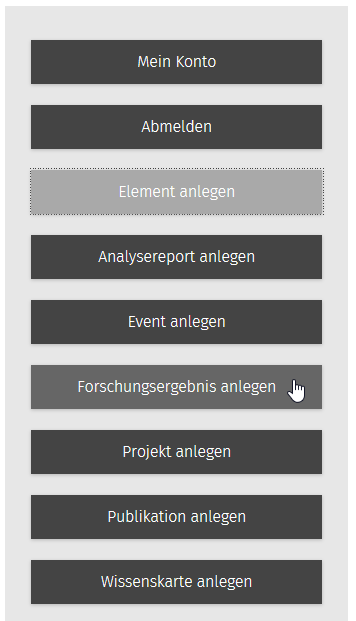
\includegraphics[height=0.20\textheight]{images/example_nodecreationlinks}
		\caption[]{Beispiel}
		\label{fig:example_nodecreationlinks}
	\end{subfigure}
	\caption{Custom Modul node\_creation\_links}
	\label{fig:nodecreationlinks}
\end{figure}



\subsubsection{publication\_form}\label{subsub:publicationform}
publication\_form


\subsubsection{slider\_tooltip}\label{subsub:slidertooltip}
slider\_tooltip
\begin{figure}[H]
	\centering
	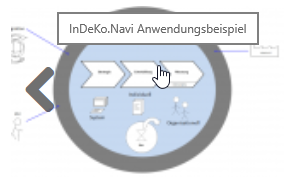
\includegraphics[height=0.10\textheight]{images/example_slidertooltip}
	\caption{Custom Modul slider\_tooltip}
	\label{fig:example_slidertooltip}
\end{figure}


\subsubsection{user\_profile\_elements\_overview}\label{subsub:userprofileelementsoverview}
user\_profile\_elements\_overview
\begin{figure}[H]
	\centering
	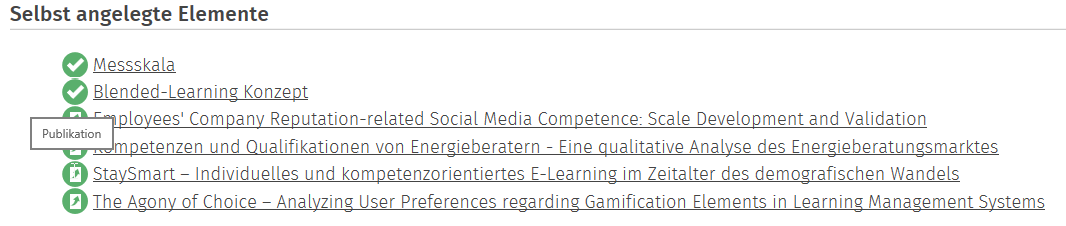
\includegraphics[width=0.80\linewidth]{images/example_userprofile}
	\caption{Custom Modul user\_profile\_elements\_overview}
	\label{fig:example_userprofile}
\end{figure}




\newpage
\subsection{Drupal Customizing}\label{sub:drupal_customizing}


\subsubsection{Darstellung der Suchergebnisse}\label{subsub:suchergebnisse}
Darstellung der Suchergebnisse
\begin{figure}[H]
	\centering
	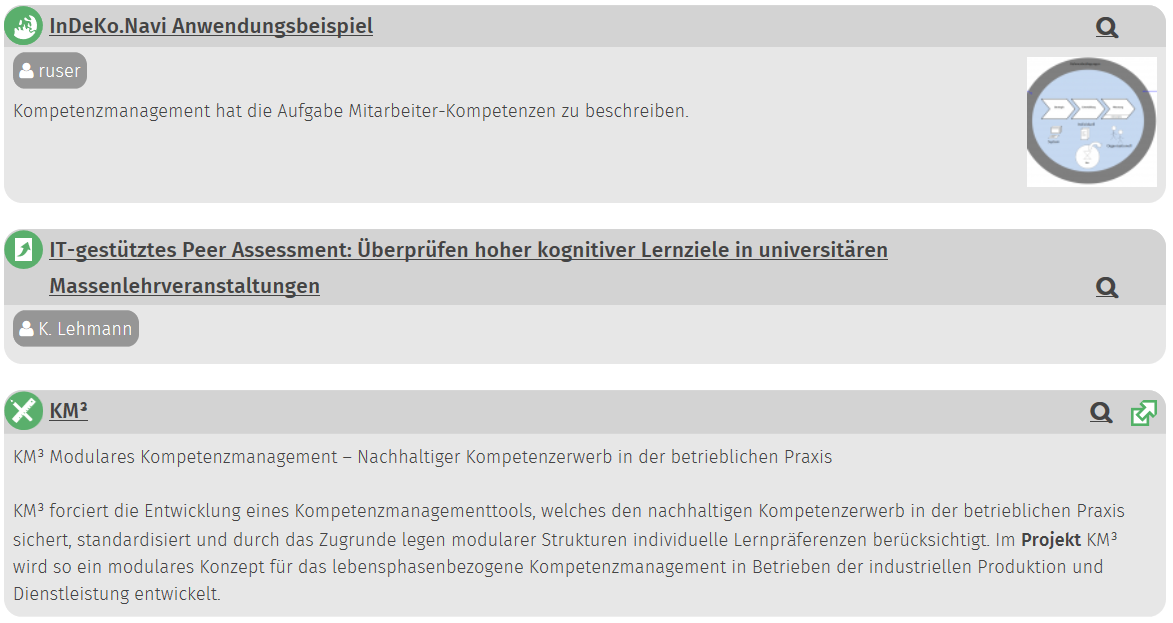
\includegraphics[height=0.20\textheight]{images/example_searchresult}
	\caption{Darstellung der Suchergebnisse}
	\label{fig:example_searchresult}
\end{figure}


\subsubsection{Slider mit Wissenskarten als Startseite}\label{subsub:wkslider}
Slider mit Wissenskarten als Startseite
\begin{figure}[H]
	\centering
	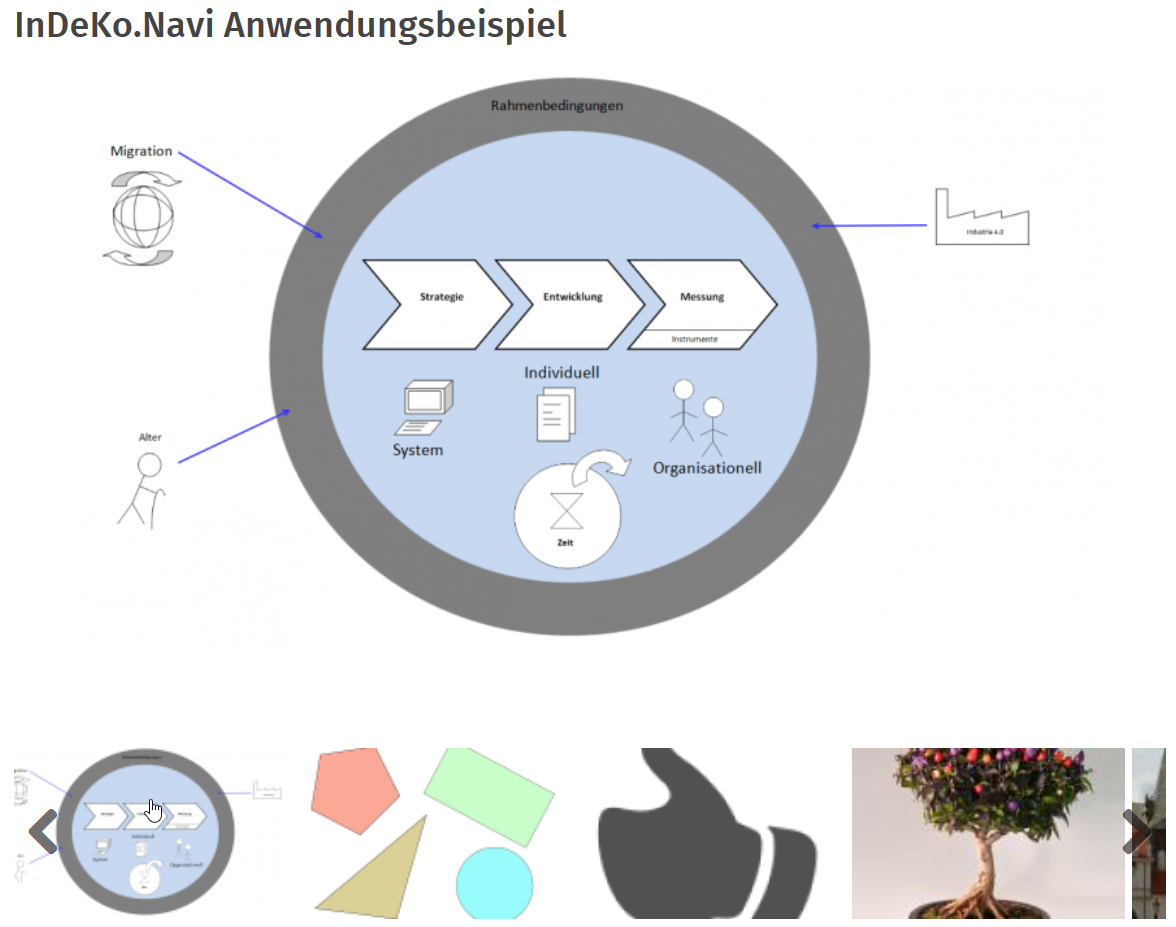
\includegraphics[height=0.20\textheight]{images/example_slider}
	\caption{Slider mit Wissenskarten als Startseite}
	\label{fig:example_slider}
\end{figure}


\subsubsection{Apache Solr Search}\label{subsub:apachesolr}



\subsubsection{CSS / Design / ???}\label{subsub:cssdesign}
CSS / Design / ???




\newpage
\section{Fehler und deren Lösungen}\label{sec:problems}

\begin{itemize}[parsep=0pt, itemsep=5.0pt plus 2.0pt minus 1.0pt, leftmargin=*]
	\item \textit{ERROR 2006 (HY000) at line [\dots]: MySQL server has gone away}

	MySQL Konfiguration (my.ini | XAMPP -> MySQL -> Config)
	\textbf{max\_allowed\_packet} erhöhen (\zB auf \enquote{32M}).


	\item \textit{Fatal error: Allowed memory size of [\dots] bytes exhausted (tried to allocate [\dots] bytes) in [\dots]}

	PHP Konfiguration (php.ini | XAMPP -> Apache -> Config)
	\textbf{memory\_limit} hochsetzen .


	\item \textit{PDOException: SQLSTATE[HY000] [2002] Es konnte keine Verbindung hergestellt werden, da der Zielcomputer die Verbindung verweigerte. in lock\_may\_be\_available()}

	MySQL Server nicht gestartet oder abgestürzt.


	\item \textit{PDOException: SQLSTATE[42000]: Syntax error or access violation: 1118 The size of BLOB/TEXT data inserted in one transaction is greater than 10\% of redo log size. Increase the redo log size using innodb\_log\_file\_size.}

	MySQL Konfiguration (my.ini | XAMPP -> MySQL -> Config)
	\textbf{innodb\_log\_file\_size} erhöhen.


	\item \textit{Warning: file\_get\_contents(): http:// wrapper disabled in the server configuration by allow\_url\_fopen = 0 in \_local\_parse\_js\_file()}

	Drupal Konfiguration zur settings.php \textbf{ini\_set('allow\_url\_fopen', 1);} hinzufügen.


	\item \textit{User Warning: The following module is missing from the file system: [\dots]}

	Fehler wurde nach Upgrade auf die neuere Drupal Version angezeigt, siehe \url{https://www.drupal.org/node/2487215}.
	Betroffene Module neu zu installieren / deinstallieren oder extra Module, die den Fehler beheben sollten halfen nicht. Nur manueller Eingriff in die Datenbank führte zum Erfolg: \lstinline| "DELETE from system where name = 'old_module1' AND type = 'module';"|

	\item \dots \todo{was noch?}
\end{itemize}



\section{Verwendete Ressourcen und deren Lizenzen}\label{sub:license}
Dieses Kapitel listet alle Ressourcen und deren Lizenzen auf, die dem InDeKo.Navi-Portal im Laufe des Projekts hinzugefügt wurden. Es dient als Übersicht was, im Vergleich zum Ursprungsprojekt, neu hinzugekommen ist und zur Versicherung, dass immer noch alles Open Source ist.

\begin{enumerate}
	\item Drupal Contrib Module (alle \textbf{GPLv2})
	\begin{itemize}
		\item Administration menu (\url{https://www.drupal.org/project/admin_menu})
		\item Apache Solr Search (\url{https://www.drupal.org/project/apachesolr})
		\item Apache Solr Real-Time (\url{https://www.drupal.org/project/apachesolr_realtime})
		\item Field Group (\url{https://www.drupal.org/project/field_group})
		\item Fivestar (\url{https://www.drupal.org/project/fivestar})
		\item Halfstar (\url{https://www.drupal.org/project/halfstar})
		\item Voting API (\url{https://www.drupal.org/project/votingapi})
		\item Bibliography Module (\url{https://www.drupal.org/project/biblio})
		\item Chosen (\url{https://www.drupal.org/project/chosen})
		\item Conditional Fields (\url{https://www.drupal.org/project/conditional_fields})
		\item Entity Connect (\url{https://www.drupal.org/project/entityconnect}) (Problem mit Chosen, Links für neue Inhalte werden bei multiselect nicht hinter den chosen Elementen angeordnet. \textbf{Provisorischer Fix in \enquote{entityconnect.js} vom Entity Connect Modul})
		\item Field Validation (\url{https://www.drupal.org/project/field_validation})
		\item Display Suite (\url{https://www.drupal.org/project/ds})
		\item jQuery Autosize (\url{https://www.drupal.org/project/jquery_autosize}) \textbf{Fixed Contrib Modul: Library pattern, Drupal behaviours mussten angepasst werden}
		\item Corresponding Entity References (\url{https://www.drupal.org/project/cer}) (alpha version)  \todo{cer und elements nicht mehr benötigt?}
		\item Elements (\url{https://www.drupal.org/project/elements})
	\end{itemize}

	\item JavaScript Bibliotheken
	\begin{itemize}
		\item imgmap (\url{https://github.com/maschek/imgmap})  \textbf{GPLv2}
		\item Maphilight (\url{https://github.com/kemayo/maphilight}) \textbf{MIT}
		\item Image Map Resize (\url{https://github.com/davidjbradshaw/image-map-resizer}) \textbf{MIT}
		\item qTip\textsuperscript{2} (\url{http://qtip2.com/}) \textbf{GPLv2 \& MIT}
		\item Chosen (\url{https://harvesthq.github.io/chosen/}) \textbf{MIT}
		\item Autosize (\url{http://www.jacklmoore.com/autosize/}) \textbf{MIT}
	\end{itemize}

	\item Bilder, Grafiken, Symbole, Sounds, \dots\label{sub:license_images}
	\begin{itemize}
		\item Apache Solr (\url{http://lucene.apache.org/solr/}) \textbf{Apache License 2.0}
		\item Font Awesome Fonts (\url{http://fontawesome.io/license/}) \textbf{SIL OFL 1.1}
		\item Font Awesome CSS (\url{http://fontawesome.io/license/}) \textbf{MIT}
		\item Alle Bilder für Beispielwissenskarten \textcolor{red}{\textbf{Lizenz nicht geprüft}}
	\end{itemize}

	\item Erweiterungen indeko7-Theme (vgl. \cref{fig:structuretheme})
	\begin{itemize}
		\item \textit{global.atlas.css} enthält alle Design Anpassungen am Portal durch das Atlas-Projekt
		\item Unterordner \textit{images/atlas} enthält alle für das Atlas-Projekt erstellten svg Grafiken (von Carlo Frisch erstellt, aus E-Mail vom 5.12.2016)
		\item \textit{js/node-wissenskarte-comments-style.js}, \textit{template/comment--node-wissenskarte.tpl.php} und \textit{template.php}
	\end{itemize}

	\item Entwickelte Drupal-Custom-Module (siehe \cref{sub:custom_modules})
	\begin{itemize}
		\item form\_wissenskarte\_module, comments\_shortener, imagemap\_resizer, jq\_maphilight, morphsearch, morphsearch\_csv\_export, morphsearch\_sort, node\_creation\_links, publication\_form, slider\_tooltip, user\_profile\_elements\_overview
	\end{itemize}
\end{enumerate}


\section{Offene Punkte}


\glsaddall
% Abkürzungsverzeichnis
\printglossary[type=\acronymtype,title = Abkürzungsverzeichnis]

% Glossar
\printglossary

%\newpage
%\printbibliography
%\bibliography{atlas}
\end{document}